\documentclass[a4paper,12pt]{report}
\usepackage[utf8]{vietnam}
\usepackage{amsmath}
\usepackage{amsfonts}
%\usepackage{enumitem}
\usepackage{enumerate}
%\usepackage{amssymb}
\usepackage{graphicx}
\usepackage{caption}
%\usepackage{cases}
\usepackage{fancybox}
\usepackage{multirow}
\usepackage{longtable}
\usepackage{listings}
\usepackage[nottoc]{tocbibind}
\usepackage{indentfirst}
\usepackage[english]{babel}
\usepackage{float}
\PassOptionsToPackage{hyphens}{url}\usepackage{hyperref}  
\usepackage[left=3cm, right=2.00cm, top=2.00cm, bottom=2.00cm]{geometry}
%\lstset{
   %keywords={break,case,catch,continue,else,elseif,end,for,function,
   %   global,if,otherwise,persistent,return,switch,try,while},
%   language = Java,
%   basicstyle=\ttfamily \fontsize{12}{15}\selectfont,   
	% numbers=left,
%   frame=lrtb,
%tabsize=3
%}
\hypersetup{
    colorlinks,
    citecolor=black,
    filecolor=black,
    linkcolor=blue,
    urlcolor=red 
}
%\setlength{\parskip}{0.6em}
\addto\captionsenglish{
 \renewcommand\chaptername{Phần}
 \renewcommand{\contentsname}{Mục lục} 
 \renewcommand{\listtablename}{Danh sách bảng}
 \renewcommand{\listfigurename}{Danh sách hình vẽ}
 \renewcommand{\tablename}{Bảng}
 \renewcommand{\figurename}{Hình}
 \renewcommand{\bibname}{Tài liệu tham khảo}
}

\newtheorem{definition}{Định nghĩa}[chapter]
%\newtheorem{lema}{Bổ đề}[chapter]
%\newtheorem{theorem}{Định lý}[chapter]

\begin{document}
\thispagestyle{empty}
\thisfancypage{
\setlength{\fboxrule}{1pt}
\doublebox}{}

\begin{center}
{\fontsize{16}{19}\fontfamily{cmr}\selectfont TRƯỜNG ĐẠI HỌC BÁCH KHOA HÀ NỘI\\
VIỆN CÔNG NGHỆ THÔNG TIN VÀ TRUYỀN THÔNG}\\
\textbf{------------*******---------------}\\[1cm]

\includegraphics[scale=0.13]{hust.jpg}\\[1.3cm]
{\fontsize{32}{43}\fontfamily{cmr}\selectfont BÁO CÁO}\\[0.1cm]
{\fontsize{38}{45}\fontfamily{cmr}\fontseries{b}\selectfont MÔN HỌC}\\[0.2cm]
{\fontsize{20}{24}\fontfamily{phv}\selectfont Hình học tính t	oán}\\[0.3cm]
{\fontsize{18}{20}\fontfamily{cmr}\selectfont \emph{Đề tài: Lập kế hoạch vận di chuyển cho robot}}\\[2cm]
\hspace{-5cm}\fontsize{14}{16}\fontfamily{cmr}\selectfont \textbf{Nhóm sinh viên thực hiện:}\\[0.1cm] 
\begin{longtable}{l c c}
Nguyễn Tuấn Đạt & 20130856 & CNTT2.02-K58 \\
Phan Anh Tú &   20134501 & CNTT2.01-K58\\
Đặng Quang Trung & 20134145 & CNTT2.03-K58 \\
\end{longtable}
\vspace{0.5cm}
\hspace{-6cm}\fontsize{14}{16}\fontfamily{cmr}\selectfont \textbf{Giảng viên hướng dẫn:}\\[0.1cm]
\hspace{-2.7cm}\fontsize{14}{16}\fontfamily{cmr}\selectfont PGS-TS.Huỳnh Thị Thanh Bình \\[3cm]
\fontsize{16}{19}\fontfamily{cmr}\selectfont Hà Nội 5--2017
\end{center}
\newpage
\pdfbookmark{\contentsname}{toc}
\tableofcontents
%\listoftables
%\listoffigures

\chapter{Mở đầu}
Một trong những mục đích cơ bản của ngành robot là thiết kế ra những con robot tự động, những con robot có khả năng tự động lập kế hoạch cho sự di chuyển của nó. Để có thể lập kế hoạch di chuyển, một con robot cần biết về môi trường xung quanh, những trướng ngại vật cần phải tránh. Và bài toán lập kế hoạch di chuyển cho robot là bài toán khó, vì vậy cần có một vài giả sử để làm đơn giản hóa bài toán: 
\begin{itemize}
\item Giả sử bài toán lập kế hoạch vận chuyển cho robot trong không gian hai chiều, với các chướng ngại vật là các đa giác, và robot cũng là một đa giác. 
\item Giả sử môi trường xung quanh robot là tĩnh, tức là không có người đi lại trên đường di chuyển của robot, các chướng ngại vật là cố định.
\end{itemize}


\section{Không gian làm việc, không gian cấu hình}
$R$ là robot di chuyển trong không gian 2 chiều (không gian làm việc), với tập $S = \{P_1, ...., P_t\}$ các chướng ngại vật. Giả sử rằng $R$ là một đa giác. Vị trí của robot có thể định nghĩa bởi một vector. Ta ký hiệu $\mathcal{R}(x,y)$ đại diện cho vector vị trí các đỉnh của robot (Điểm $(x,y)$ được gọi là điểm tham chiếu). Ví dụ robot có các đỉnh: $(1,-1), (1,1), (0,3), (-1,1), (-1,-1)$ thì $\mathcal{R}(6,4)$ sẽ đại diện cho vector vị trí của robot khi các đỉnh đa giác của robot ở các vị trí lần lượt là: $(7,3), (7,5), (6,7), (5,5), (5,3)$\\[0.6em]
Giả sử robot có thể thay đổi hướng của nó thông qua phép quay, vì vậy ta cần định nghĩa thêm một tham số ($\phi$) để biểu diễn hướng của robot. Ký hiệu $\mathcal{R}(x,y,\phi)$ xác định vị trí và hướng của robot, trong đó $(x,y)$ là điểm tham chiếu, $\phi$ là góc quay ngược chiều kim đồng hồ so với vị trí thẳng (vị trí chưa quay của robot)\\[0.6em]
Không gian các tham số của một robot $\mathcal{R}$ thường được gọi là không gian cấu hình ($\mathcal{C}(\mathcal{R})$). Một điểm $p$ trong không gian cấu hình đó sẽ tương ứng với vị trí nào đó $\mathcal{R}(p)$ của robot trong không gian làm việc.
\par Ví dụ điểm $(x,y,\phi)$ trong không gian cấu hình sẽ tương ứng với vị trí $\mathcal{R}(c,y,\phi)$ trong không gian làm việc. Không gian cấu hình là không gian $\mathbb{R}^2\times[0:360)$ (không phải không gian Euclidean 3 chiều) do chiều quay của robot là từ 0 đến 360 độ.
\par Không gian làm việc của là không gian thực tế mà robot di chuyển còn không gian cấu hình là không gian các tham số của robot (điểm tham chiếu, hướng của robot). Một đa giác (hình của robot) trong không gian làm việc sẽ được biểu diễn bởi một điểm trong không gian cấu hình và mọi điểm trong không gian cấu hình tương ứng với một vài vị trí thực của robot trong không gian làm việc.\\[0.6em]
Như vậy bằng cách xác định các giá trị cho các tham số xác định vị trí (hay nói cách khác bằng cách xác định một điểm trong không gian cấu hình) ta có thể xác định được vị trí của robot. Nhưng không phải tất cả các điểm trong không gian cấu hình sẽ xác định vị trí hợp lệ của robot. Đó là các điểm tương ứng với vị trí của các chướng ngại vật trong $S$. Ta gọi phần không gian trong không gian cấu hình chứa các điểm như vậy là không gian cấm (Ký hiệu $\mathcal{C}_{forb}(\mathcal{R},S$). Phần còn lại của không gian cấu hình bao gồm các điểm tương ứng với các vị trí tự do (không vướng các chướng ngại vật) được gọi là không gian tự do (Ký hiệu $\mathcal{C}_{free}(\mathcal{R},S)$).
\par Một đường đi của robot trong không gian làm việc sẽ tương đương với một đường cong trong không gian cấu hình (nối các điểm trong không gian cấu hình tương ứng với các vị trí trên đường đi của robot trong không gian làm việc) (Hình \ref{fig_path})
\begin{figure}[H]
\label{fig_path}
\centering
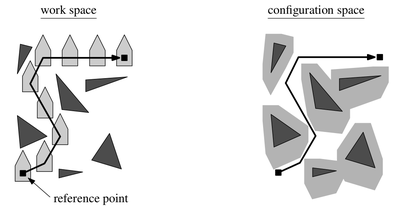
\includegraphics[scale=1]{path.png}
\caption{Đường đi trong không gian làm việc và không gian cấu hình}
\end{figure}
\par Một chướng ngại vật $\mathcal{P}$ trong không gian làm việc tương ứng một tập các điểm $p$ trong không gian cấu hình 

\section{Minkowski Sums}
Trong phần trước chúng ta đã giải quyết vấn đề lập kế hoạch cho robot điểm, chúng ta tính một bản đồ hình thang của không gian trống và sử dụng bản đồ này để lên kế hoạch. Phương pháp tương tự có thể sử dụng nếu như robot là một đa giác. Có một sự khác biệt làm cho việc xử lý robot đa giác trở nên khó khăn hơn: Hình dạng không gian các chướng ngại vật là không giống nhu trong không gian làm việc. Vì vậy chúng ta sẽ bắt đầu tìm hiểu các hình dạng không gian của biến thể đa giác robot. Trong phần tiếp theo, chúng ta sẽ mô tả cách tính nó, để chúng ta có thể sử dụng nó để lên kế hoạch cho chuyển động của robot.
\\
Chúng ta giả sử rằng robot $\Re$ là lồi, và chúng ta cũng giả sử rằng các chướng ngại vật là lồi. Chúng ta sử dụng $\Re(x,y)$ để biểu diễn vị trí của $\Re$ tham chiếu cho điểm ở vị trí (x,y). Không gian câu hình của chướng ngại vật, hoặc C-obstacle, của một chướng ngại vật   P và robot R được định nghĩa như một tập các điểm trong không gian cấu hình tương  đương với vị trí của R giao với P. Vì vậy nếu chúng ta định nghĩa C-obstacle của P bởi CP, chúng ta có
\begin{displaymath}
CP = \{(x,y): \Re(x,y)\cap P \neq \emptyset \}
\end{displaymath}
\begin{minipage}[b]{0.45\linewidth}
\begin{center}
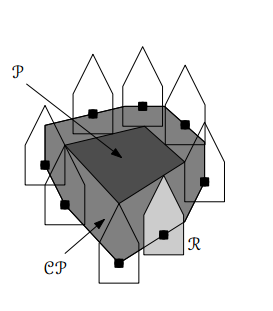
\includegraphics[width=0.8\linewidth]{1.png}
\captionof{figure}{MINKOWSKI SUMS}
\end{center}
\end{minipage}
\begin{minipage}[b]{0.45\linewidth}
\begin{center}
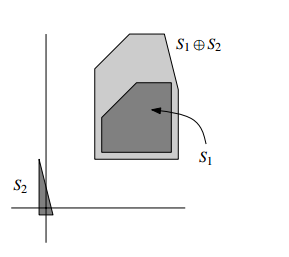
\includegraphics[width=0.8\linewidth]{2.png}
\captionof{figure}{MINKOWSKI SUMS $S_1$ và $S_2$}
\end{center}
\end{minipage}
 \\
Chúng ta có thể hình dung hình dạng của CP bằng cách trượt R dọc theo ranh giới bao ngoài của P; Đường cong bắt đầu từ điểm R là ranh giới của CP. \\ \\
Chúng ta có thể mô tả điều này bằng 1 cách khác đó là sử dujg kí pháp của \textit{Minkowski sums}. Minkowski sum của 2 tập $S_1 \subset R^2$ và $S_2 \subset R^2$, định nghĩa bằng $S_1 \oplus S_2$ được biểu diễn như:
\begin{displaymath}
S_1 \oplus S_2 := \{ p + q: p \in S_1, q\in S_2\},
\end{displaymath}
Ở đây p + q biểu diễn tổng vector của các vector P và q, có nghĩa là nếu $p = (p_x,p_y)$ và $q = (q_x,q_y)$ chúng ta có
\begin{displaymath}
p + q := (p_x + q_x, p_y + q_y)
\end{displaymath}
Bởi vì một đa giác là một tập mặt phăng được  định nghĩa bởi Minkowski sums cũng được áp dụng cho chúng. \\ \\
Để có thể biểu diễn C-obstacles như Minkowski sums, chúng ta cần thêm một ký hiệu. Ví dụ điểm $p = (p_x,p_y)$ chúng ta định nghĩa $-p:= (-p_x,-p_y)$, và tập S chúng ta định nghĩa $-S:= {-p : p \in S}$. Hay nói cách khác, chúng ta có $-S$ bởi việc phản ánh S về ban đầu. Chúng ta sẽ có định lý.\\ \\
\textbf{Định lý: } Cho $\Re$ là một mặt phẳng, robot dich và cho  P là một chướng ngại vật. Sau đó C-obstacle của P là P $\oplus (-\Re(0,0))$. \\ \\
\textit{Chứng minh.} Chúng ta phải chứng minh rằng $\Re(x,y)$ giao với P nếu và chỉ nếu chúng ta có $(x,y) \in P \oplus (-\Re(0,0)).$\\ \\
Đầu tiên, Giả sử rằng $\Re(x,y)$ giao với P, và cho $q = (q_x,q_y)$ là một điểm giao. Từ q $\in \Re(x,y)$ chúng ta có $(q_x -x , q_y - y) \in \Re(0,0)$ hoặc bằng $(-q_x + x, -q_y + y)\in -\Re(0,0)$.Bởi vì chúng ta cũng có $q \in P$,nên $(x,y) \in P \oplus (-\Re(0,0))$.\\ \\
Ngược lại, cho $(x,y) \in P \oplus (-R(0,0))$. Sau đó có điểm $(r_x,r_y) \in \Re(0,0)$ và $(p_x,p_y)\in P$ sao cho $(x,y) = (p_x - r_x, p_y - r_y)$ hay nới cách khác là $p_x = r_x + x$ và $p_y = r_y + y$. Điều này $\Re(x,y)$ giao với P.\\ \\
Vì vậy một mặt phẳng robot dịch $\Re$, C-abstacles là Minkowski sums của các chướng ngại vật và $-\Re(0,0)$. \\ \\
Trong phần còn lại của phần này chúng ta sẽ rút ra một số tính chất hữu ích của các khoản tiền Minkowski và phát triển một thuật toán để tính toán chúng. Chúng ta bắt đầu với một quan sát đơn giản về những điểm cực đoan về các khoản tiền của Minkowski \\ \\
\textbf{Quan sát: }Cho P và $\Re$ là 2 đối tượng trong mặt phẳng, và cho $CP := P \oplus \Re$. Điểm cực trị trong hướng d trên CP là tổng các điểm cực trị theo hướng d trên P và R.\\
\begin{figure}[h]
\begin{center}
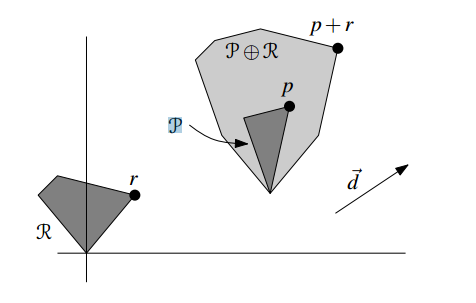
\includegraphics[width=0.5\linewidth]{5.png}
\caption{An extreme point on a Minkowski sum is the sum of extreme points}
\end{center}
\end{figure}
\textbf{Định lý: } Cho P và $\Re$ là đa giác lồi với n và m cạnh tương ứng. Sau đó Minkowski sum $P \oplus \Re$ là một đa giác lồi với số cạnh n + m. \\ \\
\textit{Chứng minh} Độ lồi của Minkowski sum của hai tập lồi theo định nghĩa. \\ \\
Để thấy được độ phức tạp của Minkowski sum là tuyến tính, xem xét cạnh e của $P \oplus \Re$. Cạnh này là cực theo hướng bình thường bên ngoài của nó. Vì vậy nó phải tạo bới điểm trên P và $\Re$ là một điểm cực trị có cùng hướng. Hơn nữa, ít nhất một điểm trong các P và R phải có một cạnh đó là cực theo hướng đó. Chúng ta sẽ đính phí cho cạnh e này. Cách này thì mỗi cạnh e sẽ được tính phí ít nhất 1 lần. Vì vậy tổng số cạnh nhiều nhất là n + m. \\
Vì vậy, tổng hợp Minkowski của hai đa giác lồi là lồi và có độ phức tạp tuyến tính. Nhưng có nhiều hơn: ranh giới của hai Minkowski sum có thể gchỉ iao nhau một cách rất đặc biệt. \\
Xem xét hai đôi tượng phẳng $o_1$ và $o_2$, mỗi mặt đều bị chặn bởi một đường cong khép kín đơn giản. Cặp điểm $o_1, o_2$ được gọi là 1 cặp pseudodiscs nếu bao của chúng $\partial o_1$ và $\partial o_2$ giao nhiều nhất 2 điểm.\\
\begin{figure}[h]
\begin{center}
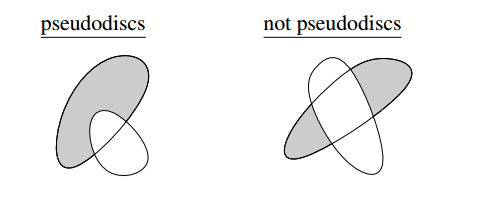
\includegraphics[width=0.5\linewidth]{6.png}
\caption{The pseudodisc property}
\end{center}
\end{figure} \\
Trong các tình huống thoái hoá khi các ranh giới có sự chồng chéo lên một chiều chẳng hạn thì định nghĩa này không hoàn toàn đủ. Do đó, chúng ta xác định chính xác $o_1$, $o_2$ là một cặp pseudodiscs nếu có điều kiện sau: $\partial o_1$ $\cap$ int($o_2$) được nối và $\partial o_2$ $cap$ int($o_1$) được nối. Một tập các đối tượng, mỗi đối tượng được bao bới một đường cong đóng được gọi là tập của pseudodisc nếu tất cả các điểm của đối tuowjnng trong tập là một cặp pseudodics. Ví dụ tâp của pseuodiscs là taajo của discs, và tập hợp các ô vuông song song trục.\\  \\
Xem xét 2 đa giác P và P'. Chúng ta nới rằng giao điểm $p \in \partial P \cap \partial P'$ là boundary crossing nếu như $\partial $ P ngang qua vùng nội địa của P' đến phần ngoài ở p. Đa giác pseudodiscs thỏa mãn những tính chất sau:\\ \\
\textbf{Quan sát: }Một cặp của đa giác pseudodiscs P,P' xác định nhiều nhất hai ranh giới giao cắt  \\
Dưới đây chúng ta sẽ chứng minh rằng một  tập các  Minkowski sum tạo thành một tập các pseudodisc. Nhưng trước tiên, chúng ta cần thêm một sự quan sát về các hướng và điểm cực trị trên các cặp đa giác lồi với các không gian lộn xộn. Chúng ta nói rằng một đa giác là nhiều cực trị  trong một hướng $\overrightarrow{d}$ hơn một đa giác khác nếu điểm cực trị của nó nằm ở hướng xa hơn các điểm cực trị của đa giác khác. Ví dụ, một đa giác cực trị hơn ở hướng x dương nếu các điểm cực phải của nó nằm bên phải các điểm cực đại của đa giác khác \\ \\
Chúng tôi sẽ xem xét các điểm cực trị cho các hướng khác nhau. Chúng ta mô hình tập tất cả các hướng bằng vòng tròn đơn vị có tâm ở gốc: một điểm p trên đơn vị tròn biểu diễn hướng được đưa ra bởi vector từ gốc đến p. Trong khoảng từ hướng $\overrightarrow{d_1}$ đến hướng $\overrightarrow{d_2}$ được xác định như hướng tương ứng với các điểm trong vòng tròn ngược chiều kim đồng hồ từ điểm biểu diễn cho $\overrightarrow{d_1}$ đến điểm biểu diễn cho $\overrightarrow{d_2}$. Lưu ý rằng khoảng từ $\overrightarrow{d_1}$ đến $\overrightarrow{d_2}$ là không giống như dải từ $\overrightarrow{d_2}$ đến $\overrightarrow{d_1}$. 
\begin{figure}[h]
\begin{center}
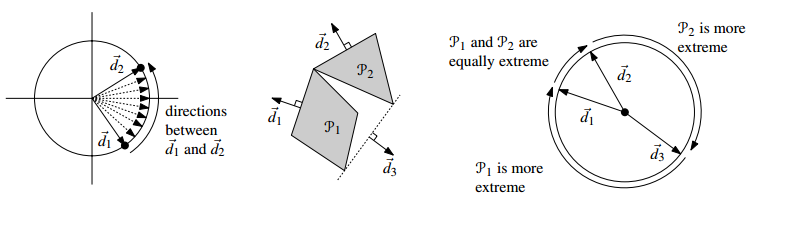
\includegraphics[width=0.9\linewidth]{7.png}
\caption{One convex polygon is more extreme
than another for a connected range of
directions}
\end{center}
\end{figure} \\
\textbf{Quan sát: } Cho $P_1$ và $P_2$ là đa giác lồi với phần nội dời. Cho $\overrightarrow{d_1}$ và $\overrightarrow{d_2}$ là hướng trong $P_1$ nhiều cực trị hơn $P_2$. Hoăc một trong hai $P_1$ là cực trị hơn $P_2$ ở tất cả các hướng trong khoảng từ $\overrightarrow{d_1}$ đến $\overrightarrow{d_2}$ hoặc trong khoảng tù $\overrightarrow{d_2}$ đến $\overrightarrow{d_1}$. \\ 
Bây giờ chúng ta đã sẵn sàng để chứng minh rằng Minkowski sum là pseudodiscs.\\ \\
\textbf{Định lý:} Cho $P_1$ và $P_2$ là hai đa giác lồi với nội rời rạc, và để $\Re$ là một đa giác lồi khác. Sau đó, hai Minkowski sum  $P_1 \oplus \Re$ và $P_2 \oplus \Re$ là các pseudodisc.
\textit{Chứng minh.} Xác định $CP_1: = P_1 \oplus \Re$ và $CP_2 := P_2 \oplus \Re$. Theo tính đối xứng, nó đủ để chứng minh rằng $\partial CP_1 \cap $ int($CP_2$) được kết nối. \\ \\
Giả sử $\partial CP_1 \cap$ int ($CP_2$) là không kết nối. Sau đó sẽ có 4 hướng xem kẽ $\overrightarrow{d_p}, \overrightarrow{d_q},\overrightarrow{d_r},\overrightarrow{d_s}$ có hướng ra ngoài của điểm p,q,r,s $\in \partial CP_1$ xuất hiện  theo thứ tự nhất định $\partial CP_1$ với p,r $\in$ int($CP_2$) và q,s $\notin$ int($CP_2$) sao cho $CP_2$  trực trị hơn $CP_1$ theo hướng $\overrightarrow{d_p}$ và $\overrightarrow{d_s}$.Từ quan sát 4 theo $P_1$ cực trị hơn $P_2$ trong hướng $\overrightarrow{d_p}$ và $\overrightarrow{d_r}$ và không cực trị hơn trong hướng $\overrightarrow{d_q}$ và $\overrightarrow{d_s}$ dẫn đến mâu thuẫn quan sát 13.7. Kết quả này hữu ích khi trộn 2 định lí. \\
\begin{figure}[h]
\begin{center}
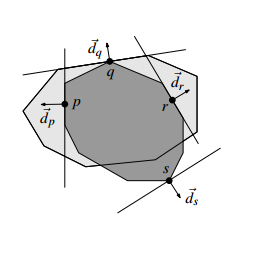
\includegraphics[width=0.4\linewidth]{8.png}
\end{center}
\end{figure}
\\  \\
\textbf{Định lý: }  Cho S là một tập của đa giác lồi pseudodiscs với tổng số cạnh là n. Độ phức tạp của chúng 2n. \\
\begin{figure}[h]
\begin{center}
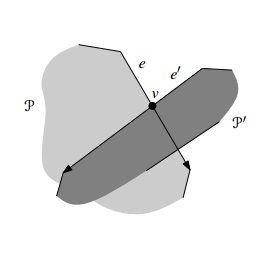
\includegraphics[width=0.4\linewidth]{9.png}

\end{center}
\end{figure}
\\
\textit{Chứng minh.} Chúng ta chứng minh ràng buộc bằng cách tính tất cả các đỉnh của liên kết tới một đỉnh pseudodisc theo cách sao cho bất kỳ điểm đỉnh pseudodisc nào được tính phí nhiều nhất hai lần. Điều này dẫn đến một ràng buộc của 2n về sự phức tạp của sự kết hợp. \\ \\
Việc tính phí được thực hiện như sau. Có hai loại đỉnh trong ranh giới liên kết: các đỉnh pseudodisc và các điểm giao cắt của nội có hai cạnh pseudodisc. \\ \\
Bây giờ hãy xem xét một đỉnh hợp v là giao điểm của một cạnh e của một pseudodisc $P \in S$ và một cạnh e' của pseudodisc $P' \in S$.Sau đó $e \cap e'$  là một boundary crossing.Vì vây quan sát 6 hoăc e không có boundary crossing khác $\partial P$ hoặc e' không có boundary crossing khác với $\partial P$. Giả sử để mà không mất tổng quát rằng e không có crossing khác với $\partial P'$. Bắt đầu $e \cap e'$, e ở nội của $P'$. Bởi vì e không ngang qua $\partial P'$ lần thứ 2, chúng ta phải chạm tới 1 điểm cuối của e trước chúng ta chạm vào ngoài của $P'$. Chúng ta sẽ tính phí v đến điểm cuối này của e. \\ \\
Nếu chúng ta tính theo cách này, thì mỗi đỉnh pseudodisc của anypseudodisc P sẽ bị tính phí nhiều nhất hai lần. \\ \\
Đầu tiên hãy xem xét trường hợp v không nằm trong nội thất hoặc trên ranh giới của bất kỳ pseudodisc P'. Mặt khác, rõ ràng v là một đỉnh kết hợp, và nó chỉ tính riêng.Tiếp theo hãy xem xét trường hợp v nằm trong nội của một số pseudodisc P.Điều này có nghĩa là v nằm trong nội của hợp. Bây giờ hãy theo hai cạnh của P đến v cho đến khi đạt được ranh giới liên kết tại một điểm crossing với một cạnh khác; Hai đường giao nhau, nếu chúng tồn tại, là những đường nối duy nhất có thể bị tính vào v.Cuối cùng, nếu v nằm trên ranh giới của một số pseudodisc P', v có thể tự tính và (tương tự như trường hợp v ở trong một pseudodisc nội) bởi hai lần đầu tiên qua hai cạnh của nó. Nó chỉ có thể được tính từ cả cạnh của nó, tuy nhiên, khi các cạnh đến từ v vào bên trong của liên kết của các pseudodiscs. Trong trường hợp đó, v không phải là đỉnh kết hợp và nó sẽ không bị tính phí. Do đó, trong mọi trường hợp, v được tính nhiều nhất hai lần.  \\ \\
Chúng ta đưa ra một thuật toán để tính tổng của Minkowski hai đa giác lồi P và R. Một thuật toán rất đơn giản là sau. Đối với mỗi cặp v, w của các đỉnh, với v $\in$ P và w $\in$ R, tính v + w. Tiếp theo, tính phần bao lồi của tất cả các sums này. Thuật toán này không hiệu quả khi đa giác có nhiều đỉnh, bởi vì nó nhìn vào mỗi cặp đỉnh.Dưới đây đưa ra một thuật toán thay thế, đó là dễ thực hiện.\\
\begin{figure}[h]
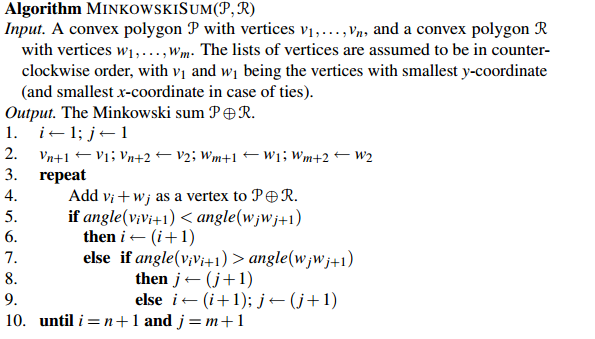
\includegraphics[width=0.85\linewidth]{ag1.png}
\end{figure}
\\
MINKOWSKISUM chạy trong thời gian tuyến tính, bởi vì tại mỗi lần thực hiện lặp lại hoặc i hoặc j được tăng lên và không phải là khó khăn để chứng minh chúng sẽ không được tăng sau khi đạt đến các giá trị n +1 và m + 1.  \\ \\
\textbf{Định lý:} Tổng của Minkowski hai đa giác lồi với đỉnh n và m, tương ứng, có thể được tính trong thời gian O (n + m). \\ \\
Điều gì xảy ra nếu một hoặc cả hai đa giác không lồi? Câu hỏi này không phải là khó để trả lời nếu chúng ta nhận ra rằng sự bình đẳng sau đây giữ cho bất kỳ bộ $S_1, S_2,$ và $S_3$:
\begin{displaymath}
S_1 \oplus (S_2 \cup S_3) = (S_1 \oplus S_2) \cup (S_1 \oplus S_3).
\end{displaymath}
Bây giờ hãy xem xét tổng của Minkowski của một đa giác không lồi P và đa giác lồi với các đỉnh n và m.
\begin{displaymath}
P \oplus \Re = \cup_{i = 1}^{n-2}t_i \oplus \Re
\end{displaymath}
Vì $t_i$ là một tam giác và $\Re$ đa giác lồi với đỉnh m, ta biết rằng $t_i \oplus \Re$ là đa giác lồi với tối đa m + 3 đỉnh. Hơn nữa, các hình tam giác có liên kết rời nhau, vì vậy việc tập Minkowski sum là một tập các pseudodisc. Do đó, độ phức tạp của  hợp của chúng là tuyến tính trong tổng độ phức tạp của chúng. Có nghĩa là độ phức tạp của $P \oplus \Re$ là O(nm). \\
\begin{figure}[h]
\begin{center}
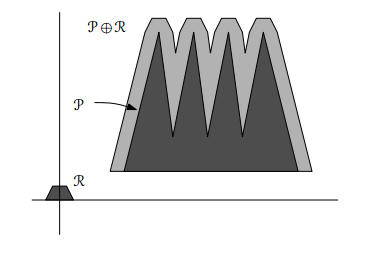
\includegraphics[width=0.6\linewidth]{10.png}
\caption{The Minkowski sum of a non-convex
and a convex polygon}
\end{center}
\end{figure}\\
Cận trên của độ phức tạp của một đa giác không lồi và đa giác lồi là chặt chẽ trong trường hợp xấu nhất.Để thấy điều này, hãy xem xét một đa giác P với $\lfloor n/2 \rfloor$ đỉnh hướng lên trên và một đa giác nhỏ hơn R là nửa trên của một bình thường có (2m-2)-gon. Minkowski sum của các đa giác này cũng sẽ có $\lfloor n/2 \rfloor$ đột biến, mỗi đỉnh có m đỉnh tại đỉnh của nó. \\ \\
Để ràng buộc sự phức tạp của Minkowski sum của hai đa giác không lồi P và R, chúng ta tính tam giác cả hai đa giác. Chúng ta nhận được một tập hợp n-2 tam giác $t_i$, và một tập hợp các tam giác m-2 $u_j$.Minkowski sum của P và $\Re$ bây giờ là hợp của các Minkowski sum các cặp $t_i, u_j$. Mỗi tổng $t_i \oplus u_j$ có độ phức tạp là hằng số. Do đó, $P \oplus \Re$ là hợp của đa giác (n-2)(m-2).Có nghĩa là tổng độ phức tạp của $P \oplus \Re$ là $O(n^2m^2)$. Một lần nữa, ràng buộc này là chặt chẽ trong trường hợp xấu nhất: có đa giác không lồi mà Minkowski sum thực sự có độ phức tạp $\Theta(n^2m^2)$ \\
\begin{figure}[h]
\begin{center}
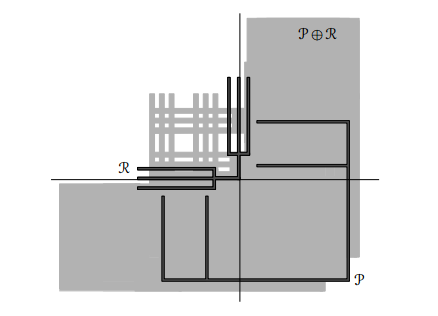
\includegraphics[width=0.6\linewidth]{11.png}
\caption{The Minkowski sum of two non-convex polygons}
\end{center}
\end{figure}\\
\textbf{Định lý:} Cho P và $\Re$ là đa giác với các đỉnh n và m, tương ứng. Độ phức tạp của Minkowski sum $P\ oplua \Re$ bị giới hạn như sau:
\begin{itemize}
\item[i, ] $O(n+m)$ nếu cả hai đa giác đều lồi.
\item[ii, ] $O(nm)$ nếu một trong các đa giác lồi và một không lồi.
\item[iii, ] s $O(n^2m^2)$ if both polygons are non-convex
\end{itemize}
\section{Translational Motion Planning}
Ở đầu trong phần kế hoạch ROBOT MOTION trước đó chúng ta đã chỉ ra rằng C-obstacle tương ứng với một trở ngại $P_i$ là Minkowski sum $Pi \oplus (-R)$. Hơn nữa, chúng ta đã thấy rằng các đa giác của Minkowski đa giác lồi là các pseudodisc. Chúng ta sử dụng điều này để chứng minh kết quả chính đầu tiên của chúng tôi về vấn đề quy hoạch chuyển động, trong đó nêu rõ rằng sự phức tạp của không gian trống của một robot biến đổi là tuyến tính. \\ \\
\textbf{Định lý 9: }Cho R là một robot lồi độ phức tạp hằng số, dịch trong một tập S các chướng ngại vật đa giác không giao nhau với tổng số n cạnh. Sau đó, độ phức tạp của không gian cấu hình miễn phí $C_{free}(R, S)$ là $O(n)$. \\ \\
\textit{Chứng minh: }Đầu tiên chúng ta tính toán từng đa giác chướng ngại vật. Chúng ta có một tập hợp $O (n)$ hình tam giác, và do đó lồi, các chướng ngại xen kẽ nhau. Không gian cấu hình tự do là bổ sung của sự hợp bơi C-obstacles của tam giác này. Bởi vì robot có độ phức tạp liên tục, những C-obstacles có độ phức tạp hằng số, và theo định lý 8, chúng tạo thành một tập các pseudodisc. Đầu tiên chúng ta tính toán từng đa giác trở ngại. Chúng ta có một tập hợp O (n) hình tam giác, và do đó lồi, những chướng ngại với sự xen kẽ nhau. Không gian cấu hình miễn phí là bổ sung của sự kết hợp của C-chướng ngại của tam giác này. Bởi vì robot có độ phức tạp liên tục, những trở ngại của C có độ phức tạp liên tục, và theo định lý 13.8, chúng tạo thành một tập các pseudodisc. Định lý 9 bây giờ có nghĩa rằng sự kết hợp có sự phức tạp tuyến tính. \\ \\
Cho $P_1, \ldots , P_n$ định nghĩa các tam giác chúng ta có được khi sắp xếp các chướng ngại vật. Chúng ta tính
\begin{displaymath}
C_{ford} = \cup_{i = 1}^nCP_i = \cup_{i = 1}^nP_i \oplus(-\Re(0,0)).
\end{displaymath}
\begin{figure}[h]
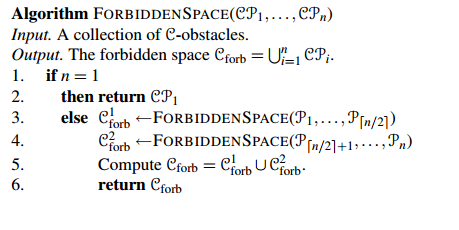
\includegraphics[width=0.7\linewidth]{ag2.png}
\end{figure}
\\
\textbf{Bổ đề } Không gian cấu hình $C_{free}$ của robot lồi liên tục chuyển đổi giữa các tập đa giác với n cạnh tổng thể có thể tính trong thời gian $O(n\log^2n)$. \\ \\
Bây giờ chúng ta đã tính được không gian trống, chúng ta có thể tiếp tục giống như trong Phần 13.2: chúng ta tính toán một bản đồ hình thang của không gian trống, cùng với lộ trình. Với vị trí bắt đầu và vị trí mục tiêu của robot R, chúng ta tìm thấy một đường dẫn như sau. Đầu tiên, chúng ta lập bản đồ bắt đầu và vị trí mục tiêu cho các điểm trong không gian cấu hình. Sau đó chúng ta tính toán đường đi giữa hai điểm này qua không gian trống bằng bản đồ hình thang và bản đồ đường, như được mô tả trong phần 13.2. Cuối cùng, chúng ta ánh xạ đường dẫn đến một đường dẫn cho R trong không gian làm việc. Định lý tiếp theo tóm tắt kết quả của những nỗ lực của chúng tôi. \\ \\ 
\textbf{Định lý: } Cho $\Re$ là một robot lồi độ phức tạp liên tục dịch. Trong một tập S phân chia của các chướng ngại vật đa giác n cạnh trong tổng số. Chúng ta có thể tiền sử lí S trong $O (n\log^2n)$ thời gian dự kiến, chẳng hạn như giữa bất kỳ vị trí bắt đầu và vị trí mục tiêu một đường dẫn không va chạm cho $\Re$, nếu tồn tại, có thể được tính trong $O(n)$
\begin{thebibliography}{9} 

\end{thebibliography}


\end{document}
